\documentclass[../../../../main.tex]{subfiles}
\begin{document}

\section{User Input}
\subsection{Shared Layer Access}
Within Java there is a standard dictionary like structure called a \texttt{Map} which we can use to store the layers. More specifically a \texttt{Map}\cite{mapJava} is actually a interface and the specific class we will be using to store the layers is called a \texttt{HashMap}\cite{hashmapJava} (It can be said that \texttt{HashMap} inherits \texttt{Map}). I am using a \texttt{HashMap} since it is lightweight and simple to use\. With this information I implemented the \texttt{ShareLayers} class:
\begin{minted}[
frame=lines,
framesep=2mm,
linenos,
breaklines,
fontsize = \fontsize{9}{9}
]{java}
package application;

import java.util.ArrayList;
import java.util.HashMap;
import java.util.Map;

import javafx.beans.property.BooleanProperty;
import javafx.beans.property.SimpleBooleanProperty;
import layer.Layer;

public class ShareLayers {

	// attributes
	private Map<Integer, Layer> layers;
	private BooleanProperty changeLayers;

	// methods
	// constructor
	public ShareLayers() {
		// initialize attributes
		layers = new HashMap<Integer, Layer>();
		changeLayers = new SimpleBooleanProperty(true);
	}

	// add a layer
	public void putLayer(int ID, Layer layer) {
		// add the layer
		this.layers.put(ID, layer);
		// notify the plot pane to draw again
		this.changeLayers.set(!this.changeLayers.get());
	}

	// remove a layer
	public void removeLayer(int ID) {
		// remove the layer
		this.layers.remove(ID);
		// notify the plot pane to draw again
		this.changeLayers.set(!this.changeLayers.get());
	}

	// return a list of layers
	public ArrayList<Layer> getLayers() {
		return new ArrayList<Layer>(this.layers.values());
	}

	// return the property which notifies the plotpane
	public BooleanProperty getChangeLayers() {
		return changeLayers;
	}

}
\end{minted}
\newpage\noindent
Since the plot pane will need to be connected to the shared layer access, I created a method called \texttt{setShareLayerStore()} which sets up the connection between the plot pane and the shared layer access. I also gave it two new attributes, a reference to the shared layer access to get the list of layers \texttt{shareLayerStore} and the boolean property \texttt{changeLayers} that the shared layer access will bind with. Here is the implementation of the new method:
\begin{minted}[
frame=lines,
framesep=2mm,
linenos,
breaklines
]{java}
// set up the shared layer access
public void setShareLayerStore(ShareLayers shareLayerStore) {
	// set the shared layer access attribute
	this.shareLayerStore = shareLayerStore;
	// bind and set the value for the property
	this.changeLayers.set(this.shareLayerStore.getChangeLayers().get());
	this.changeLayers.bind(this.shareLayerStore.getChangeLayers());
	// create a listener to execute when the plot pane needs to draw again
	ChangeListener<Object> redrawListener = (observable, oldValue, newValue) -> {
		// remove all the old layers
		this.layers.clear();
		// add all the new layers
		for (Layer l : shareLayerStore.getLayers()) {
			this.addLayer(l);
		}
		// draw the functions again
		try {
			drawAll();
		} catch (StackOverflowException | StackUnderflowException | UnequalBracketsException
				| InterruptedException e) {
			// error in drawing a function
			e.printStackTrace();
		}
	};
	// bind the listener to the property
	this.changeLayers.addListener(redrawListener);
}
\end{minted}
\newpage
\subsection{Expression Box}
Before creating the expression box and its controller class I created a dummy input pane class that contained all its methods and attributes, none of which were properly implemented, so that I wouldn't get any compilation errors. I first created the FXML file using scene builder. This is what I produced:
\begin{figure}[H]
	\begin{center}
		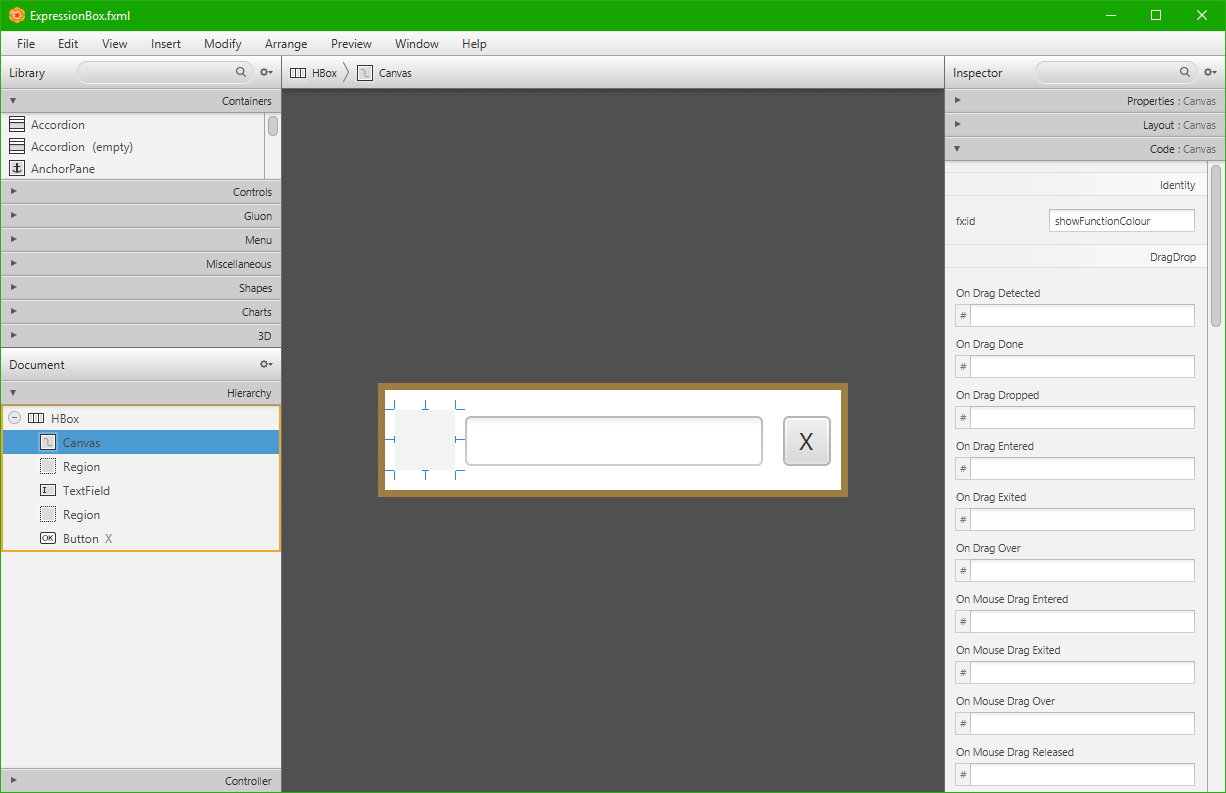
\includegraphics[width=0.45\textwidth]{images/expressionBox}
	\end{center}
	\caption{Creating the Expression Box in Scene Builder}
\end{figure}
For the button to show/hide the function I decided to use a canvas to achieve the effect. It gives me finer control about the colour of the button and is easier to manipulate. I showed my stakeholders this and Matthew said that he \textit{``liked the simple design''}. The FXML for the expression box is shown below:
\begin{minted}[
frame=lines,
framesep=2mm,
linenos,
breaklines,
fontsize = \fontsize{9}{9}
]{xml}
<?xml version="1.0" encoding="UTF-8"?>

<?import javafx.geometry.Insets?>
<?import javafx.scene.canvas.Canvas?>
<?import javafx.scene.control.Button?>
<?import javafx.scene.control.TextField?>
<?import javafx.scene.layout.HBox?>
<?import javafx.scene.layout.Region?>

<HBox alignment="CENTER" xmlns="http://javafx.com/javafx/8.0.171"
	xmlns:fx="http://javafx.com/fxml/1"
	fx:controller="application.ExpressionBoxController">
	<children>
		<Canvas fx:id="showFunctionColour" height="30.0" width="30.0">
			<HBox.margin>
				<Insets left="5.0" />
			</HBox.margin>
		</Canvas>
		<Region HBox.hgrow="ALWAYS" />
		<TextField fx:id="inputTxt">
			<HBox.margin>
				<Insets left="5.0" right="5.0" />
			</HBox.margin>
		</TextField>
		<Region />
		<Button fx:id="removeBtn" mnemonicParsing="false" text="X">
			<HBox.margin>
				<Insets left="5.0" right="5.0" />
			</HBox.margin>
		</Button>
	</children>
	<padding>
		<Insets bottom="10.0" top="10.0" />
	</padding>
</HBox>
\end{minted}
\newpage
I then created the controller class. I introduced a few new methods such as the \texttt{changeColor()} method. This one is triggered when the canvas is clicked and shows/hides the function and updates the visual aid. The \texttt{changeLayer()} method is called whenever the input text changes or the user clicks on the show/hide canvas. It parses the input text determines whether or not it is a function in $x$, $y$, the Normal Distribution, or none of those. It then creates a layer for that specific function and then adds it to the shared access layer through the input pane. The code for the rest of this class was quite simple to implement and it is below:
\begin{minted}[
frame=lines,
framesep=2mm,
linenos,
breaklines,
fontsize = \fontsize{9}{9}
]{java}
package application;

import java.io.IOException;
import java.net.URL;
import java.util.ResourceBundle;

import exceptions.StackOverflowException;
import exceptions.StackUnderflowException;
import exceptions.UnequalBracketsException;
import javafx.beans.property.SimpleStringProperty;
import javafx.beans.property.StringProperty;
import javafx.fxml.FXML;
import javafx.fxml.Initializable;
import javafx.scene.canvas.Canvas;
import javafx.scene.canvas.GraphicsContext;
import javafx.scene.control.Button;
import javafx.scene.control.TextField;
import javafx.scene.paint.Color;
import layer.ExplicitXFunctionCartesianLayer;
import layer.ExplicitYFunctionCartesianLayer;
import layer.Layer;
import structures.Expression;
import structures.NormalDistribution;

public class ExpressionBoxController implements Initializable {

	// attributes
	private int ID;
	private GraphicsContext gc;
	private boolean functionVisiblity = true;
	private Color color;
	private StringProperty functionText = new SimpleStringProperty();
	private InputPane inputPane;
	// FXML components
	@FXML
	private TextField inputTxt;
	@FXML
	private Button removeBtn;
	@FXML
	private Canvas showFunctionColour;

	// methods
	// empty constructor
	public ExpressionBoxController() {
	}

	@Override
	// called when initialized a pseudo constructor of sorts
	public void initialize(URL arg0, ResourceBundle arg1) {
		// bind the input to a string property in the class to manipulate
		this.functionText.set(inputTxt.textProperty().getValueSafe());
		this.functionText.bind(inputTxt.textProperty());
		// add a listener so that every time it changes the layer is updated
		this.functionText.addListener(event -> {
			try {
				changeLayer();
			} catch (StackOverflowException | StackUnderflowException | UnequalBracketsException e) {
				e.printStackTrace();
			}
		});
		// if the remove button is clicked call the remove method
		this.removeBtn.setOnAction(event -> {
			try {
				remove();
			} catch (IOException e) {
				e.printStackTrace();
			}
		});
		// create the canvas to show the color of the function
		this.gc = this.showFunctionColour.getGraphicsContext2D();
		this.gc.setLineWidth(2);
		// when the canvas is clicked change its color by calling the change Color
		// method
		this.showFunctionColour.setOnMouseClicked(event -> {
			try {
				changeColor();
			} catch (StackOverflowException | StackUnderflowException | UnequalBracketsException e) {
				e.printStackTrace();
			}
		});
	}

	// update the layer
	private void changeLayer() throws StackOverflowException, StackUnderflowException, UnequalBracketsException {
		// only change the layer if is not hidden by the user
		if (functionVisiblity) {
			Layer l;
			String f = this.functionText.getValueSafe();
			// if the function is empty remove the layer
			if (f.length() == 0) {
				inputPane.removeLayer(ID);
				return;
			}
			// if it begins with normal create a normal distribution layer
			if (f.startsWith("Normal(")) {
				f = f.replaceAll("Normal\\(", "");
				f = f.replaceAll("\\)", "");
				String[] variables = f.split(",");
				// μ;
				double μ = 0;
				// σ2;
				double σ2 = 1;
				// get the values for the mean and variance
				μ = new Expression(variables[0], 'x').evaluate(0);
				σ2 = new Expression(variables[1], 'x').evaluate(0);
				// create the function
				NormalDistribution normalDist = null;
				normalDist = new NormalDistribution(μ, σ2);
				// create the layer with the specific color
				l = new ExplicitXFunctionCartesianLayer(normalDist);
				l.setColor(color);
				// add the layer to the shared layer access
				inputPane.putLayer(this.ID, l);
				// terminate this function
				return;
			}
			// determine the whether it is an explicit x or y function by counting their
			// respective instances
			// count the number of x instances
			int xInstances = f.length() - f.replaceAll("x", "").length();
			// count the number of y instances
			int yInstances = f.length() - f.replaceAll("y", "").length();
			if (xInstances > 0 && yInstances > 0) { // if it contains both x and y remove it since it is implicit
				inputPane.removeLayer(ID);
				return;
			} else if (yInstances > 0) { // if it contains only y create a explicit function in y
				l = new ExplicitYFunctionCartesianLayer(f);
				l.setColor(color);
				inputPane.putLayer(this.ID, l);
			} else if (xInstances > 0) { // if it contains only x create a explicit function in x
				l = new ExplicitXFunctionCartesianLayer(f);
				l.setColor(color);
				inputPane.putLayer(this.ID, l);
			}
		} else { // if the function is hidden then remove the layer
			inputPane.removeLayer(ID);
		}
	}

	// show/hide the function and update the visual identifier
	private void changeColor() throws StackOverflowException, StackUnderflowException, UnequalBracketsException {
		// clear the canvas
		gc.clearRect(0, 0, showFunctionColour.getWidth(), showFunctionColour.getHeight());
		if (!functionVisiblity) {
			// fill it in color if showing the function
			gc.fillRect(0, 0, showFunctionColour.getWidth(), showFunctionColour.getHeight());
		}
		// draw a black border so it is clickable
		gc.strokeRect(0, 0, showFunctionColour.getWidth(), showFunctionColour.getHeight());
		// negate the visibility since it has changed
		functionVisiblity = !functionVisiblity;
		// remove or add the layer to show/hide it
		changeLayer();
	}

	// remove itself from the input pane
	private void remove() throws IOException {
		this.inputPane.removeExpressionBox(this.ID);
	}

	// set the id
	public void setID(int iD) {
		ID = iD;
	}

	// get the id
	public int getID() {
		return ID;
	}

	// set the parent input pane
	public void setInputPane(InputPane inputPane) {
		this.inputPane = inputPane;
	}

	// set the color of the function
	public void setColor(Color color) {
		this.color = color;
		gc.setStroke(color);
		gc.setFill(color);
		gc.fillRect(0, 0, showFunctionColour.getWidth(), showFunctionColour.getHeight());
	}

}
\end{minted}
\newpage
\subsection{Input Pane}
I then implemented the input pane class.
\newpage
\end{document}